\renewcommand*{\arraystretch}{1.5}
\noindent\begin{tabularx}{17cm}{|p{1.95cm}|X|}
	\hline
	number      & 1                                                          \\ \hline
	title       & Friends with certain name                                                           \\ \hline
	\multicolumn{2}{|c|}{ 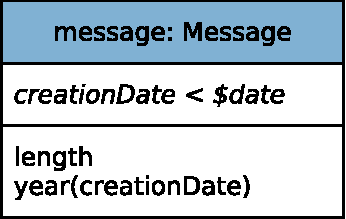
\includegraphics[scale=\patternscale,margin=0cm .2cm]{patterns/q01}} \\ \hline
	description & Given a start Person, find Persons with a given first name that the
start Person is connected to (excluding start Person) by at most 3 steps
via Knows relationships. Return Persons, including summaries of the
Persons workplaces and places of study.
 \\ \hline
	
	parameters  &
	\renewcommand*{\arraystretch}{1.0}
	\vspace{-1.8ex}{\begin{tabularx}{14.2cm}{|c|l|p{2cm}|Y|} \hline
	\cellcolor{black!70} \color{white} $\mathsf{1}$ & \varname{Person.id} & \cellcolor{gray!20} \vartype{ID} & \\ \hline
	\cellcolor{black!70} \color{white} $\mathsf{2}$ & \varname{Person.firstName} & \cellcolor{gray!20} \vartype{String} & \\ 
	\end{tabularx}} \\ \hline
	result      &
	\renewcommand*{\arraystretch}{1.0}
	\vspace{-1.8ex}{\begin{tabularx}{14.2cm}{|c|l|p{2cm}|Y|} \hline
	\cellcolor{black!70} \color{white} $\mathsf{1}$ & \varname{Person.id} & \cellcolor{gray!20} \vartype{ID} & \\ \hline
	\cellcolor{black!70} \color{white} $\mathsf{2}$ & \varname{Person.lastName} & \cellcolor{gray!20} \vartype{String} & \\ \hline
	\cellcolor{black!70} \color{white} $\mathsf{3}$ & \varname{Person.birthday} & \cellcolor{gray!20} \vartype{Date} & \\ \hline
	\cellcolor{black!70} \color{white} $\mathsf{4}$ & \varname{Person.creationDate} & \cellcolor{gray!20} \vartype{DateTime} & \\ \hline
	\cellcolor{black!70} \color{white} $\mathsf{5}$ & \varname{Person.gender} & \cellcolor{gray!20} \vartype{String} & \\ \hline
	\cellcolor{black!70} \color{white} $\mathsf{6}$ & \varname{Person.browserUsed} & \cellcolor{gray!20} \vartype{String} & \\ \hline
	\cellcolor{black!70} \color{white} $\mathsf{7}$ & \varname{Person.locationIP} & \cellcolor{gray!20} \vartype{String} & \\ \hline
	\cellcolor{black!70} \color{white} $\mathsf{8}$ & \varname{\{Person.emails\}} & \cellcolor{gray!20} \vartype{\{String\}} & \\ \hline
	\cellcolor{black!70} \color{white} $\mathsf{9}$ & \varname{\{Person.language\}} & \cellcolor{gray!20} \vartype{\{String\}} & \\ \hline
	\cellcolor{black!70} \color{white} $\mathsf{10}$ & \varname{Person-isLocatedIn->Place.name} & \cellcolor{gray!20} \vartype{String} & \\ \hline
	\cellcolor{black!70} \color{white} $\mathsf{11}$ & \varname{\{Person-studyAt->University.name, Person-studyAt->.classYear, Person-studyAt->University-isLocatedIn->City.name\}} & \cellcolor{gray!20} \vartype{\{<String, 32bitInteger, String>\}} & \\ \hline
	\cellcolor{black!70} \color{white} $\mathsf{12}$ & \varname{\{Person-workAt->Company.name, Person-workAt->.workFrom, Person-workAt->Company-isLocatedIn->Country.name\}} & \cellcolor{gray!20} \vartype{\{<String, 32bitInteger, String>\}} & \\ 
	\end{tabularx}} \\ \hline
	sort        &
	\renewcommand*{\arraystretch}{1.0}
	\vspace{-1.8ex}{\begin{tabular}{|c|l|c|} \hline
	\cellcolor{black!70} \color{white} $\mathsf{1}$ & \varname{distance from person} & \cellcolor{gray!20} $\asc$ \\ \hline
	\cellcolor{black!70} \color{white} $\mathsf{2}$ & \varname{Person.lastName} & \cellcolor{gray!20} $\asc$ \\ \hline
	\cellcolor{black!70} \color{white} $\mathsf{3}$ & \varname{Person.id} & \cellcolor{gray!20} $\asc$ \\ 
	\end{tabular}} \\ \hline
	limit       & 20                                                           \\ \hline
	choke points        &
	\multicolumn{1}{>{\raggedright}X|}{
		}\\ \hline
\end{tabularx}
\clearpage